\section{数列的极限}
\label{sec:ru-sequence-limits}
\label{sec:analysis-continuous-limits}
\label{sec:analysis-sequences-series-errors}

数列$1,1/2,1/3,\ldots$越来越接近$0$，数列$-1,1,-1,1,\ldots$则在两个值之间来回交替。
直觉上前者“有极限”，后者没有；但“越来越接近”需要精确的含义，否则无法判断$(1+1/n)^n$或$\sum_{k\leq n}1/k$这类数列是否趋向某个数。
本节先用误差条件定义收敛并建立极限的运算，再给出不必事先知道极限值的存在性判别，最后描述趋向无穷和不收敛数列的尾部行为。

\subsection{收敛、发散与极限运算}
\label{sec:ru-convergence-limit-laws}

比较$(1/n)$与$((-1)^n)$，区别在于尾部。$1/n$从某一项起全部落在$0$附近任意窄的范围内；$((-1)^n)$的偶数项都等于$1$，奇数项却始终离$1$有距离$2$。
所以“接近一个数”必须约束后面的\emph{每一项}。只要求“各项离$a$越来越近”也不够：$1+1/n$离$0$越来越近，却始终大于$1$。
合适的要求是：无论事先给定多小的正误差，从某一项起，后面每一项与$a$的距离都小于这个误差。

\begin{definition}[数列的极限]
\label{def:ru-sequence-limit}
设$(a_n)$为实数列，$a\in\mathbb R$。若对每个$\varepsilon>0$，都存在正整数$N$，使
\[
 n\geq N\quad\Longrightarrow\quad|a_n-a|<\varepsilon,
\]
就称$(a_n)$\term{收敛}（converge）到$a$，$a$称为它的极限，记作$\lim_{n\to\infty}a_n=a$或$a_n\to a$。没有实数极限的数列称为\term{发散}（diverge）。
\end{definition}

定义中的量词次序不能交换：先任给误差$\varepsilon$，再选取尾部起点$N$。$N$可以依赖于$\varepsilon$，误差要求越严格，所需的起点通常越靠后。
极限也不要求某一项恰好等于$a$\scite{math-lebl-analysis1}。
例如对$a_n=1/n$，任给$\varepsilon>0$，由Archimedes性取正整数$N>1/\varepsilon$，则$n\geq N$时$|1/n-0|\leq1/N<\varepsilon$，所以$1/n\to0$。
图~\ref{fig:analysis-process-sequence-tail}把“全部尾部项”画成同一条误差带。

\begin{figure}[!htbp]
 \centering
 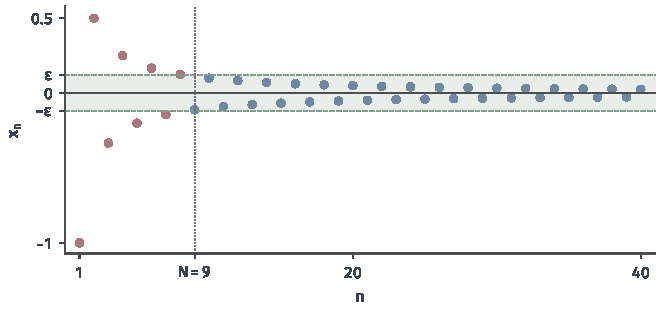
\includegraphics[width=112.0mm]{figures/01-mathematical-preliminaries-upper/00-shared/matplotlib/chapter3-concept-processes/sequence-tail.pdf}
 \caption{数列$x_n=(-1)^n/n$的前40项。绿色带为$|x_n|<0.12$，取$N=9$后，所有$n\geq9$都在带内；蓝点标记这个尾部，红点标记之前的项。尾部条件针对无限多个$n$，其成立依据是$1/n\leq1/9<0.12$，不是只检查图中有限个点。}
 \label{fig:analysis-process-sequence-tail}
\end{figure}

要说明$a_n$不收敛到$a$，须写出定义的否定：存在某个$\varepsilon_0>0$，使得无论$N$取多大，总有$n\geq N$满足$|a_n-a|\geq\varepsilon_0$。
对$((-1)^n)$，取$\varepsilon_0=1$：相邻两项相差$2$，不可能同时落在长度为$2$的开区间$(a-1,a+1)$内，所以它不收敛到任何$a$，是发散数列。

定义需要先给出一个候选极限$a$，那么会不会有两个候选都满足定义？不会。若$a\neq b$都是极限，取$\varepsilon=|a-b|/3$，充分靠后的项同时满足$|a_n-a|<\varepsilon$和$|a_n-b|<\varepsilon$，
三角不等式却给出$|a-b|\leq|a-a_n|+|a_n-b|<2|a-b|/3$，矛盾。所以收敛数列的极限唯一，记号$\lim a_n$表示一个确定的数。

定义只控制尾部，而尾部之前只有有限个项，因此收敛数列必有界。设$a_n\to a$，取$\varepsilon=1$得到$N$，使$n\geq N$时$|a_n|<|a|+1$；
再令$M=\max\{|a_1|,\ldots,|a_{N-1}|,|a|+1\}$，就有$|a_n|\leq M$对所有$n$成立。
反过来不成立，$((-1)^n)$有界却不收敛。这一性质常以逆否形式使用：无界数列一定发散。

已知几个数列收敛时，由它们组合出的数列的极限可以直接算出。思路都是把新数列的误差拆成已知误差的组合。
\begin{theorem}[数列极限的四则运算]
\label{thm:ru-sequence-limit-laws}
设$a_n\to a$，$b_n\to b$，其中$a,b\in\mathbb R$，$c$为实常数，则
\[
 a_n\pm b_n\to a\pm b,\qquad ca_n\to ca,\qquad a_nb_n\to ab.
\]
若还有$b\neq0$，则充分靠后的$b_n\neq0$，并且$a_n/b_n\to a/b$。
\end{theorem}
\begin{proof}
和与差由$|(a_n\pm b_n)-(a\pm b)|\leq|a_n-a|+|b_n-b|$得到：让两个误差各小于$\varepsilon/2$即可。数乘的误差是$|c|\,|a_n-a|$，同样可以任意小。

乘积的误差含有一个变化的因子，需要用到收敛数列的有界性。取$M\geq1$使所有$|a_n|\leq M$，则
\[
 |a_nb_n-ab|=|a_n(b_n-b)+b(a_n-a)|\leq M|b_n-b|+|b|\,|a_n-a|,
\]
让$|b_n-b|<\varepsilon/(2M)$与$|a_n-a|<\varepsilon/[2(|b|+1)]$同时成立，右侧便小于$\varepsilon$。

对商，先取误差$|b|/2$，得知充分靠后的$|b_n|\geq|b|/2>0$。于是
\[
 \Bigl|\frac1{b_n}-\frac1b\Bigr|=\frac{|b_n-b|}{|b_n|\,|b|}\leq\frac{2|b_n-b|}{|b|^2}\to0,
\]
前面有限个项不影响极限，再对$a_n\cdot(1/b_n)$用乘积规则。
\end{proof}
例如把分子分母同除以$n$，得$n/(n+1)=1/(1+1/n)\to1$。分母极限为零时不能套用商的规则：$0/0$与$\infty-\infty$都不是可以直接计算的数值，须先变形。

有时一个数列不断振荡，直接控制它的误差并不方便，但能找到两个趋向同一值的上下界。
\begin{theorem}[夹逼定理]
\label{thm:analysis-sequence-squeeze}
设实数列满足：存在$N_0$使$n\geq N_0$时$a_n\leq c_n\leq b_n$，并且$a_n\to\ell$、$b_n\to\ell$，其中$\ell\in\mathbb R$，则$c_n\to\ell$。
\end{theorem}
\begin{proof}
任给$\varepsilon>0$，取$N\geq N_0$使$n\geq N$时$|a_n-\ell|<\varepsilon$且$|b_n-\ell|<\varepsilon$。于是$\ell-\varepsilon<a_n\leq c_n\leq b_n<\ell+\varepsilon$，即$|c_n-\ell|<\varepsilon$。
\end{proof}
例如$-1/n\leq(\sin n)/n\leq1/n$，所以$(\sin n)/n\to0$。

等比数列$(r^n)$是反复出现的例子，夹逼定理可以判定它的全部情形。$r=0$时显然趋于零。若$0<|r|<1$，写$1/|r|=1+h$，$h>0$。
对$n$归纳可证$(1+h)^n\geq1+nh$：$n=1$时取等号；若对$n$成立，则$(1+h)^{n+1}\geq(1+nh)(1+h)\geq1+(n+1)h$。
因此$0<|r|^n\leq1/(1+nh)<1/(nh)\to0$，再对$-|r|^n\leq r^n\leq|r|^n$用夹逼定理，得到$r^n\to0$。
$r=1$时各项恒为$1$，收敛；$r=-1$时在$\pm1$间交替，发散；$|r|>1$时同一不等式给出$|r|^n\geq1+nh$（其中$|r|=1+h$），数列无界，因而发散。
回到等比递推~\eqref{eq:prelim-geometric-recurrence}：设$e_0\neq0$，$e^{(t)}=\rho^te_0$恰在$|\rho|<1$时趋于零，在$\rho=1$时保持不变，其余情形发散。

\subsection{极限存在的判别}
\label{sec:ru-limit-existence}

定义收敛时需要先给出候选极限，但很多数列的极限值事先并不知道。下面依次利用变化方向、取值范围和尾部各项的相互接近来判断极限是否存在。

若对所有$n$都有$a_n\leq a_{n+1}$，称数列单调不减；若总有$a_n\geq a_{n+1}$，称数列单调不增，两者统称单调数列。
单调不减且有上界的数列，全部项的集合有上确界；单调性又保证后面的项一直靠近它。
\begin{theorem}[单调有界收敛定理]
\label{thm:analysis-monotone-bounded-sequence}
单调不减且有上界的实数列收敛，极限为$\sup\{a_n:n\geq1\}$；单调不增且有下界的实数列收敛，极限为$\inf\{a_n:n\geq1\}$。
\end{theorem}
\begin{proof}
设$a=\sup\{a_n:n\geq1\}$，它由确界原理保证存在。给定$\varepsilon>0$，$a-\varepsilon$不是上界，所以存在$N$使$a_N>a-\varepsilon$。
单调性使$n\geq N$时$a-\varepsilon<a_N\leq a_n\leq a$，这正是$a_n\to a$。单调不增的情形对$-a_n$应用同一论证。
\end{proof}
两个条件都不能省去：$(n)$单调却无上界，$((-1)^n)$有界却不单调。结合收敛数列的有界性，单调数列收敛当且仅当它有界。

有界数列未必收敛，但其中可能有一部分项具有共同的趋向。若$n_1<n_2<\cdots$为严格递增的正整数列，则$(a_{n_k})_{k\geq1}$称为$(a_n)$的\term{子列}（subsequence），由归纳可知$n_k\geq k$。
收敛数列的每个子列都收敛到同一极限：若$n\geq N$时$|a_n-a|<\varepsilon$，则$k\geq N$时$n_k\geq k\geq N$，同一误差界仍然适用。
\begin{theorem}[Bolzano--Weierstrass定理]
\label{thm:analysis-bounded-subsequence}
有界实数列必有收敛子列。
\end{theorem}
\begin{proof}
设$|a_n|\leq M$。从包含全部项的闭区间$I_0=[-M,M]$出发，将它平分；两半中至少有一半含有无穷多个下标对应的项，选出这一半。
重复平分与选择，得到嵌套闭区间$I_0\supseteq I_1\supseteq\cdots$，其中每个$I_k$都含有无穷多项，长度为$2M\cdot2^{-k}$。
由于每个$I_k$都含有无穷多项，可以依次选取下标$n_1<n_2<\cdots$使$a_{n_k}\in I_k$。
由$2^k\geq k+1$，区间长度可以任意小，闭区间套性质给出唯一公共点$c$。$a_{n_k}$与$c$都在$I_k$中，所以$|a_{n_k}-c|\leq2M\cdot2^{-k}\to0$。
\end{proof}
“有界”只能保证子列收敛，不能保证整列收敛：$((-1)^n)$的偶数项子列收敛到$1$，奇数项子列收敛到$-1$，整列却发散。

单调条件并不适用于所有收敛数列。不知道候选极限时，还可以检查尾部各项是否彼此接近。满足
\[
 \forall\varepsilon>0,\quad\exists N,\quad\forall m,n\geq N,\quad|a_m-a_n|<\varepsilon
\]
的数列称为\term{柯西数列}（Cauchy sequence）。这个条件只涉及数列自身的项，不需要知道极限是多少。
\begin{theorem}[柯西收敛准则]
\label{thm:analysis-cauchy-convergence}
实数列收敛，当且仅当它是柯西数列。
\end{theorem}
\begin{proof}
收敛数列是柯西数列：若$n\geq N$时$|a_n-a|<\varepsilon/2$，则对$m,n\geq N$有$|a_m-a_n|\leq|a_m-a|+|a-a_n|<\varepsilon$。

反过来，先说明柯西数列有界：取误差$1$得到$N$，所有$n\geq N$都满足$|a_n-a_N|<1$，前面有限项另取最大绝对值即可。
由Bolzano--Weierstrass定理，可取子列$a_{n_k}\to a$。给定$\varepsilon>0$，选$N$使$m,n\geq N$时$|a_m-a_n|<\varepsilon/2$，再选$k$使$n_k\geq N$且$|a_{n_k}-a|<\varepsilon/2$。
于是每个$n\geq N$都有$|a_n-a|\leq|a_n-a_{n_k}|+|a_{n_k}-a|<\varepsilon$。
\end{proof}
充分性经过收敛子列，因而仍然依赖确界原理。在有理数中，$\sqrt2$的十进制截断$1,1.4,1.41,\ldots$是柯西数列，却没有有理数极限。

验证柯西条件时，可把两个较晚的项之间的距离估计为逐步变化的总和：对$m>n$，
\begin{equation}
 |a_m-a_n|\leq\sum_{k=n}^{m-1}|a_{k+1}-a_k|.
 \label{eq:analysis-cauchy-tail-bound}
\end{equation}
只看相邻两项不够，因为中间的步数也在增加。设$a_1=0$、$a_{k+1}-a_k=1/k$，每一步都趋于零；但$a_{2n}-a_n=\sum_{k=n}^{2n-1}1/k$共有$n$项，每项都大于$1/(2n)$，
所以$a_{2n}-a_n>1/2$。它不是柯西数列，因而发散。这里的$a_{n+1}$正是第~\ref{sec:analysis-series}节调和级数的前$n$项和。

\subsection{无穷极限、上极限与下极限}
\label{sec:ru-infinite-limits-limsup}

数列$(n)$发散，但它的发散方式很确定：越过任何有限界以后不再回头。为记录这种趋向，规定$a_n\to+\infty$表示对每个实数$M$，都存在$N$使$n\geq N$时$a_n>M$；
$a_n\to-\infty$则要求最终都有$a_n<M$。趋向$\pm\infty$的数列仍是发散数列，$\pm\infty$不是实数极限。
把这两个符号加入实数，得到扩展实数$\overline{\mathbb R}=\mathbb R\cup\{-\infty,+\infty\}$。其中的运算只在不引起歧义时定义，例如$a+(+\infty)=+\infty$（$a$为实数）；
$\infty-\infty$、$0\cdot\infty$与$\infty/\infty$都没有定义，因为不同的数列组合会给出不同结果，如$(n+1)-n\to1$而$2n-n\to+\infty$。

不收敛的数列仍然可以考察尾部的上下边界。逐渐舍去前项时，尾部下确界只会上升，尾部上确界只会下降，因此可以用单调数列的极限记录它们。
\begin{definition}[上极限与下极限]
\label{def:analysis-liminf-limsup}
对实数列$(a_n)$，定义
\[
 \liminf_{n\to\infty}a_n=\lim_{n\to\infty}\inf_{k\geq n}a_k,\qquad
 \limsup_{n\to\infty}a_n=\lim_{n\to\infty}\sup_{k\geq n}a_k,
\]
分别称为\term{下极限}（limit inferior）与\term{上极限}（limit superior）。尾部无上界时$\sup_{k\geq n}a_k=+\infty$，无下界时尾部下确界为$-\infty$。
\end{definition}
右侧尾部下确界随$n$单调不减，尾部上确界随$n$单调不增，所以两个极限都在扩展实数中存在：单调有界时由单调有界收敛定理得到有限极限，无界时趋于相应的无穷。
每个尾部的下确界不超过同一尾部的上确界，所以总有$\liminf a_n\leq\limsup a_n$。

上、下极限恰好刻画了通常的收敛。若二者都等于有限数$a$，给定$\varepsilon>0$，充分靠后的尾部下确界大于$a-\varepsilon$、尾部上确界小于$a+\varepsilon$，
夹在中间的每个尾部项都满足$|a_n-a|<\varepsilon$，即$a_n\to a$。反之若$a_n\to a$，则$n\geq N$时尾部全落在$(a-\varepsilon,a+\varepsilon)$内，尾部的上下确界都在$[a-\varepsilon,a+\varepsilon]$中。
同理，两者都等于$+\infty$恰好对应$a_n\to+\infty$，都等于$-\infty$对应$a_n\to-\infty$。

两者不相等时，它们记录了数列尾部来回摆动的范围。$((-1)^n)$的下极限为$-1$、上极限为$1$；$((-1)^nn)$的下极限为$-\infty$、上极限为$+\infty$；
$(n(1+(-1)^n))$的奇数项为$0$、偶数项为$2n$，下极限为$0$、上极限为$+\infty$。
对有界数列，上极限还是某个子列的极限：记$L=\limsup a_n$，对每个$j$先取足够晚的起点使其后的尾部上确界小于$L+1/j$，
这一尾部中又有某项大于$L-1/j$；在超过前次所选下标的位置选出这样的项，便得到趋于$L$的子列。下极限同理。
